\documentclass[a4paper, 12pt]{article}
\usepackage[utf8]{inputenc}
\usepackage{graphicx}
\graphicspath{ {images/} }
\usepackage[a4paper,left=3cm,right=3cm,top=3cm,bottom=3cm]{geometry}
\usepackage{tikz}
\usepackage{mathptmx}
\usetikzlibrary{shapes.geometric, arrows}
\usepackage{tikz}
\usetikzlibrary{positioning,shapes,fit,arrows}
\definecolor{myblue}{RGB}{56,94,141}
\usepackage{fancyhdr}
\usepackage{booktabs}
\usepackage{mathtools}
\usepackage{amsmath}
\usepackage{romannum}
\usepackage{etoolbox}
%\apptocmd{\thebibliography}{\csname phantomsection \endcsname \addtocontentsline{toc}{chapter}{\bibname}}{}{}
\usepackage{caption}
\usepackage{float}
\floatstyle{boxed}
\tikzstyle{rect} = [draw, rectangle, fill=white!=20, text width=6em, text centered, minimum height=2em]
\tikzstyle{line} = [draw, -latex']

\restylefloat{figure}
\pagestyle{fancy}
\fancyhf{}
\renewcommand{\headrulewidth}{0pt}
\fancyfoot[L]{P:F-SMR-UG / 08 / R0}
\fancyfoot[R]{\thepage}
%\title{First document}
\begin{document}

\pagenumbering{empty} 
%\begin{titlepage}
    \begin{center}
    	\pagestyle{fancy}
    	\fancyfoot[L]{P:F-SMR-UG/08/RO}
        \textbf{PUNE INSTITUTE OF COMPUTER TECHNOLOGY,}	\\
        \textbf{DHANKAWADI PUNE-43.}
        \vspace{1cm}
        
        \large
        \textbf{\textit{A}}\\
        \textbf{\textit{Seminar Report}}\\
        \textbf{\textit{On}}\\
        \vspace{0.5cm}
        \large
        \textbf{FINGERPRINT RECOGNITION}
        \linebreak
        \linebreak
		
		%\vspace{0.2cm}
		\small
		SUBMITTED BY \\
		\vspace{1cm} 
		
		\textbf{NAME: ANIKET JALAN}\\
		\vspace{0.5cm}
		\textbf{ROLL NO: 3208}\\
		\vspace{0.5cm}
		\textbf{CLASS: TE-2}\\
		\vspace{0.5cm}
		{GUIDED BY}
		
        \textbf{PROF: V.V.BAGADE }
        \vspace{1cm}
        
        
\includegraphics[scale=0.6]{pict.png}
        \vspace{1cm}
        
		\textbf{COMPUTER ENGINEERING DEPARTMENT}
		\vspace{0.5cm}
		
		\textbf{Academic Year:2017-18}
        \Large
    \end{center}
%\end{titlepage}
\pagebreak
%2
\pagenumbering{arabic}
%\begin{titlepage}
\begin{center}
	\textbf{PUNE INSTITUTE OF COMPUTER TECHNOLOGY,}	\\
	\textbf{DHANKAWADI PUNE-43.}
	\vspace{1cm}
	
	\large
	\textbf{\textit{CERTIFICATE}}
	\vspace{1cm}
	
	
\includegraphics[scale=0.6]{pict.png} 
	\linebreak
\end{center}	
	
	    
		 This is to certify that Mr.ANIKET JALAN Roll No. 3208
		 a student of T.E. (Computer Engineering Department) Batch 2017-2018, has
		 satisfactorily completed a seminar report on 
		 \textbf{"FINGERPRINT RECOGNITION"} under the guidance of prof. V. V. Bagade towards the partial fullfillment of the third year Computer Engineering \Romannum{2} of Pune University.  
		 \vspace{2cm}
		 
		\begin{center}
		\begin{table}[h]
		\begin{tabular}{ccc}
		\vspace{0.5cm}
		
		\noindent\rule{4cm}{0.4pt}    &                  & \hspace{47mm} \noindent\rule{4cm}{0.4pt}\\
		Prof.V. V. Bagade    &                        &  \hspace{52mm} Dr. R. B. Ingle\\
		\textbf{Internal Guide}      &                     &    \hspace{52mm} \textbf{Head of Department,} \\
		          &                         &       \hspace{50mm}\textbf{Computer Engineering} \\
		\end{tabular}
		\end{table}
		\end{center}
\textbf{Place: Pune}\\
Date:
 \newpage
\tableofcontents
\newpage

    \begin{center}
    
        
        \large
        \textbf{FINGERPRINT RECOGNITION}
        \linebreak

     \end{center}


\large
\textbf{ABSTRACT}
\vspace{1em}

\par
Fingerprints are widely used in daily life for more than 100 years due to its feasibility, distinctiveness, permanence, accuracy, reliability, and acceptability. Fingerprint is a pattern of ridges, furrows and minutiae, which are extracted using inked impression on a paper or sensors. Fingerprints have been used as the most popular biometric authentication and verification measure because of their high acceptability, immutability and uniqueness. Neural Network algorithm mainly consist of three main processing blocks, namely pre-processing which is based on four steps, pre-processing is used to improve image quality due to which detection become easy, it transform original image to a thinned image which is used for minutiae extraction. It is a four step process, namely normalization, enhancement, binarization and thinning. After pre-processing feature extraction is done using Minutiae Extraction and Profile Building and the last step in which extracting feature is to feed Artificial Neural Network which uses feedback forward backpropogational neural network to classify the fingerprint.\\\\
\textbf{Keywords}: fingerprint recognition; neural networks; minutiae extraction; image pre-processing; logistic sigmoid.
\section{INTRODUCTION}
\subsection{MOTIVATION}
In today’s world identity of a individual is most important thing. Fingerprint act as a important tool to identify whether the given individual is the right person or he is faking his identity. It is very important to make a device or to make a algorithm which help to identify whether the given fingerprint is of the respective individual or not. Fingerprint act as important biometric which help us to maintain security.


\subsection{LITERATURE REVIEW}
There exist many different types of algorithm for fingerprint recognition. Minutiae extraction is one of the important methods for fingerprint recognition. For extraction of points we first have to pre-process the image. Ridouane Oulhiq, Saad Ibntahir, Marouane Sebugi, Zouhair Guennoun[1] have proposed four basic steps of image pre-processing which include normalization, Fourier enhancement of image, Binarization and Thinning of image. Using these processes we are able to convert fingerprint into a image due to which we can extract points for profile building.\\\\
Sozan Abdulla Mahmood[2] proposed how to give input to neural network. He proposed to use crossing number algorithm to find ridges ending and bifurcation points. He also proposed that the input neurons will be the area of triangles of points extracted which will be unique for the individual.
\subsection{APPLICATIONS AND IDENTIFICATION OF CHALLENGES IN DOMAIN}
Fingerprint recognition can be used in various applications where security is the important concern. Fingerprint can be used in election voting system where person will be only allowed to vote if his fingerprint matches. It can be used in any application where user is given authorization only if his/her fingerprint matches. It is difficult to find ending and bifurcation points if image is not pre-processed properly and which lead to false prediction of fingerprint by neural network as points are not proper.
\section{SURVEY OF MATHEMATICAL MODELS}
Normalization [1] bring grey level values in fingerprint in desired range of values.\\\\
N(x, y) = $M+\frac{\sqrt{VAR\times (I(x,y)-M_R)^{2}} }{\sqrt{VAR_R}}$
, if I(x, y) $>$M\_R \begin{flushright}
(1)
\end{flushright}
\hspace{2cm} $M-\frac{\sqrt{VAR\times (I(x,y)-M_R)^{2}} }{\sqrt{VAR_R}}$, 
otherwise.\\\\
Where M\_R is the mean of all intensities and VAR\_R is the variance of the input image I(x, y) and M and VAR is the desired mean and intensity of image we want so the gray scale image can be standardize.\\\\
Fingerprint enhancement by Fourier Transform [1] is an important image processing tool which is used to decompose an image into its sine and cosine components and decrease some of background noise like false connection between ridges.\\\\
f(u, v) = $\sum_{x=0}^{m-1}{\sum_{y=0}^{n-1}{F(x,y)e^{-j2\pi \times 
(\frac{ux}{m}+\frac{vy}{n})}}}$
\begin{flushright}
(2)
\end{flushright}
For x = 0,1,\ldots ,m-1 and y=0,1,\ldots ,n-1.\\\\
Image is converted back into spatial domain by taking inverse of Fourier transform.\\\\
g (u,v) = $F^{-1}\lfloor F(x,y)\times \vert F(x,y)^{K}\vert \rfloor $ \begin{flushright}
(3)
\end{flushright}
now $F^{-1}(F(x,y))$ is given by\\\\
F(x,y) = $\frac{1}{mn}\sum_{u=0}^{m-1}{\sum_{v=0}^{n-1}{f(u,v)e^{-j2\pi 
\times (\frac{ux}{m}+\frac{vy}{n})}}}$ 
\begin{flushright}
(4)
\end{flushright} 
For u = 0,1,2\ldots .m-1 and v=0,1,2\ldots n-1.\\\\
Crossing number $[$2$]$ is used to find the ending and bifurcation 
points.\\\\
\textit{Cn }= $\frac{1}{2}\sum_{i=1}^{8}{\vert P_{i}-P_{i+1}\vert }$
\begin{flushright}
(5)
\end{flushright}
Where Pi is the binary pixel value in the neighbourhood of P with Pi= (0 
or 1) and P9=P1.
\section{PROPOSED MATHEMATICAL MODEL}
Consider working system to be S.\\\\
Let S = \{s,e,X,Y,Fn,Su\}\\\\
where,\\\\
s = start state= \{I\}\\\\
I = Fingerprint image\\\\
e = end state\\\\
X = set of input parameters\\\\
X= \{X1,X2,X3,X4,X5,X6\}\\\\
X1 =Simple Image\\\\
X2 = Normalised Image\\\\
X3 = Enhanced Image.\\\\
X4 =Binary Image.\\\\
X5 =Thinning Image.\\\\
X6 = Area of Triangles.\\\\
Y =set of output parameters.\\\\
Y =\{Y1,Y2,Y3,Y4,Y5,Y6\}\\\\
Y1,Y2,Y3,Y4 are output of pre-processing image. Y5 is the output of 
profile building. And Y6 is the output of neural network.\\\\
Fn = \{F1,F2,F3,F4,F5,F6\}\\\\
F1= function used to Normalised the image.\\\\
F2= function used to Enhanced the image.\\\\
F3= function used to convert image into binary.\\\\
F4= function used for thinning the image.\\\\
F5= function used for profile building.\\\\
F6= function used for recognising image using neural network.\\\\
Su= final output set=\{S1\}\\\\
S1= Fingerprint found.




\section{DESIGN AND ANALYSIS OF SYSTEM}
Fingerprint recognition requires 3 main steps for correct recognition of fingerprint. Firstly pre-processing of image is done so that the correct and clear image of fingerprint is obtained. In second step profile building is done which is used to extract minutiae. And in the last step points extracted from the second step is given input to neural network which classify whether the given individual is faking his identity or not.
\subsection{Pre-processing of image}
In pre-processing of image input image is converted into a form from which points can be easily extracted. In pre-processing first normalization is done which bring the gray scale value of image into desired range value. Than this image is enhanced by Fourier transform by converting image in sin and cosine components than multiplying each block by constant and enhanced them by multiplying constant and converting image back into spatial domain by using inverse Fourier transform. Enhanced image is than converted into binary image by converting pixel gray scale value to 0 and 1 with help of threshold value, if gray scale value is less than threshold than pixel value become 1 else it become 0. And finally thinning of image is done which make the ridges one pixel wide. Thinning algorithm is a Morphological operation that is used to remove selected foreground pixels from binary images. It preserves the topology (extent and connectivity) of the original region while throwing away most of the original foreground pixels.
\subsection{Minutiae extraction}
It help us in getting ending and bifurcation points of ridges with the help of crossing number which evaluate the neighbouring points value using formula given in equation5 and find whether given point is ending or bifurcation point. And each point is given direction based on neighbouring points pixel binary value and given point crossing number and set of ending and bifurcation point is prepared.\\\\
After extraction of points area of triangle is found based on the direction of points. Than area of triangle are arranged in descending orders and the first ten area of triangles are taken. 
\subsection{Neural Network}
Area of triangle which is obtained is given input to neural network. This 10 areas act as 10 input neuron which uses feed forward backpropagational neural network for classification purpose. Feed forward means how neurons are connected to other neuron in the next layer. Every neuron is connected with other neuron through a connection link. Each connection link is associated with a weight that has information about the input signal. This is the most useful information for neurons to solve a particular problem because the weight usually excites or inhibits the signal that is being communicated. Each neuron has an internal state, which is called an activation signal. Output signals, which are produced after combining the input signals and activation rule, may be sent to other units.\\\\
The back propagation algorithm falls into the general category  of  the  gradient  descent  algorithms,  which  intends  to  find  the  minima/maxima  of  a  function  by  iteratively  moving  in  the  direction  of  the  negative  of  a slope  of  a  function  to minimized/maximized.  The main objective is to minimize an error function. We calculate the total error at the output nodes and propagate these errors back through the network using Backpropagation to calculate the gradients. Then we use an optimization method such as Gradient Descent to ‘adjust’ all weights in the network with an aim of reducing the error at the output layer. We  get the output as yes or no whether the given fingerprint matches or not.
\begin{figure}[h]
\begin{center}
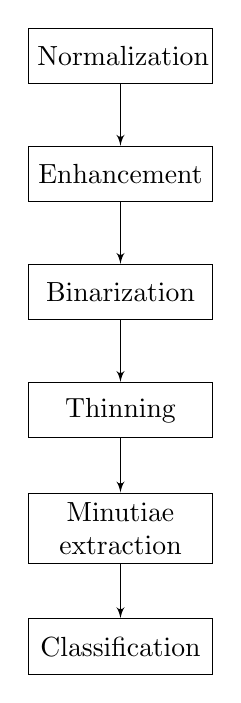
\begin{tikzpicture}[node distance=1.5cm, auto]
\node [rect] (step1) {Normalization};
\node [rect, below of=step1] (step2) {Enhancement};
\node [rect, below of=step2] (step3) {Binarization};
\node [rect, below of=step3] (step4) {Thinning};
\node [rect, below of=step4] (step5) {Minutiae extraction};
\node [rect, below of=step5] (step6) {Classification};
\path [line] (step1) -- (step2);
\path [line] (step2) -- (step3);
\path [line] (step3) -- (step4);
\path [line] (step4) -- (step5);
\path [line] (step5) -- (step6);
\end{tikzpicture}
\caption{WORK MODEL}
\label {f1}
\end{center}
\end{figure}
\section{DISCUSSION ON IMPLEMENTATION RESULTS}

\begin{table}[h!]
\centering
\begin{tabular}{|l|l|}
\hline
N(x,y) & Normalization \\
\hline
F(X,Y) & Enhancement \\
\hline 
B(x,y) & Binarization \\
\hline
T(x,y) & Thinning \\
\hline
S(X,Y) & Minutiae Extraction \\
\hline 
O & Neural Network \\
\hline
\end{tabular}
\caption{Steps of Fingerprint Recognition}
\end{table}
\begin{figure}[h!]
 \includegraphics[width=10cm,height=4cm]{output.png}
 \caption{Binarized Image}
 
\end{figure}
Binarized Image is obtained after performing first 3 steps.After binarization we can apply all the remaining process to extract feature
points and than apply ANN to classify.
\section{CONCLUSION AND FUTURE ENHANCEMENT}
Hence by using ANN we can recognise fingerprint accurate and precisely.It gives better prediction rate than any other machine learning technique. We can make prediction more accurately by enhancing the image such that we get all ridges points so that the input to the neural network is unique area of sets of the individual which ultimately leads to correct prediction of fingerprint.
\section{REFERENCES}
$[$1$]$ Sozan Abdulla Mahmood, “Fingerprint Recognition System using Support Vector       Machine and Neural Network”, (IJCSEITR), Vol.4, Issue 1, 2014, 103-110.\\\\
$[$2$]$ Ridouane Oulhiq, Saad Ibntahir, Marouane Sebugi, Zouhair Guennoun, “A Fingerprint Recognition Framework using Artificial Neural Network”, IEEE 2015, 978-1-4799-7560-0/15/\$31.\\\\
$[$3$]$ Ridouane Oulhiq, Saad Ibntahir, Marouane Sebugi, Zouhair Guennoun, “ A Fingerprint Recognition Framework using Artificial Neural Network ”,IEEE 2015, 978-1-4799-7560-0/15/$31.


\end{document}     
      